\documentclass{beamer}
\usepackage{setspace}
\usepackage{gensymb}
\singlespacing
\usepackage{amsmath}
\usepackage{bm}
%\usepackage{tikz}
%\usepackage{circuitikz}
%\usepackage{tkz-euclide}
\usepackage{cite}
\usepackage{cases}
\usepackage{subfig}
\usepackage{longtable}
\usepackage{multirow}
\usepackage{verbatim}
\usepackage{hyperref}
\usepackage{listings}
\usepackage{color}    
\usepackage{array}    
\usepackage{longtable}
\usepackage{calc}     
\usepackage{multirow} 
\usepackage{hhline}   
\usepackage{ifthen}   
\DeclareMathOperator*{\Res}{Res}

% correct bad hyphenation here
\hyphenation{op-tical net-works semi-conduc-tor}
\def\inputGnumericTable{}                                 %%

\lstset{
%language=C,
frame=single, 
breaklines=true,
columns=fullflexible
}
%\lstset{
%language=tex,
%frame=single, 
%breaklines=true
%}
\hypersetup{
    colorlinks=true,
    linkcolor=black,
    urlcolor=blue,
}
\usetheme{CambridgeUS}

\DeclareMathOperator*{\argmax}{arg\,max}
\DeclareMathOperator*{\argmin}{arg\,min}
\newtheorem{proposition}{Proposition}[section]
\newcommand{\BEQA}{\begin{eqnarray}}
\newcommand{\EEQA}{\end{eqnarray}}
\newcommand{\define}{\stackrel{\triangle}{=}}
\bibliographystyle{IEEEtran}
\providecommand{\mbf}{\mathbf}
\providecommand{\pr}[1]{\ensuremath{\Pr\left(#1\right)}}
\providecommand{\qfunc}[1]{\ensuremath{Q\left(#1\right)}}
\providecommand{\sbrak}[1]{\ensuremath{{}\left[#1\right]}}
\providecommand{\lsbrak}[1]{\ensuremath{{}\left[#1\right.}}
\providecommand{\rsbrak}[1]{\ensuremath{{}\left.#1\right]}}
\providecommand{\brak}[1]{\ensuremath{\left(#1\right)}}
\providecommand{\lbrak}[1]{\ensuremath{\left(#1\right.}}
\providecommand{\rbrak}[1]{\ensuremath{\left.#1\right)}}
\providecommand{\cbrak}[1]{\ensuremath{\left\{#1\right\}}}
\providecommand{\lcbrak}[1]{\ensuremath{\left\{#1\right.}}
\providecommand{\rcbrak}[1]{\ensuremath{\left.#1\right\}}}
\theoremstyle{remark}
\newtheorem{rem}{Remark}
\newcommand{\sgn}{\mathop{\mathrm{sgn}}}
\providecommand{\abs}[1]{\left\vert#1\right\vert}
\providecommand{\res}[1]{\Res\displaylimits_{#1}} 
\providecommand{\norm}[1]{\left\lVert#1\right\rVert}
\providecommand{\mtx}[1]{\mathbf{#1}}
\providecommand{\mean}[1]{\mathbb{E}\left[ #1 \right]}   
\providecommand{\fourier}{\overset{\mathcal{F}}{ \rightleftharpoons}}
\providecommand{\system}[1]{\overset{\mathcal{#1}}{ \longleftrightarrow}}
\newcommand{\cosec}{\,\text{cosec}\,}
\providecommand{\dec}[2]{\ensuremath{\overset{#1}{\underset{#2}{\gtrless}}}}
\newcommand{\myvec}[1]{\ensuremath{\begin{pmatrix}#1\end{pmatrix}}}
\newcommand{\mydet}[1]{\ensuremath{\begin{vmatrix}#1\end{vmatrix}}}
\renewcommand{\vec}[1]{\mathbf{\boldsymbol{#1}}}
% Theme choice:
\newcounter{saveenumi}
\newcommand{\seti}{\setcounter{saveenumi}{\value{enumi}}}
\newcommand{\conti}{\setcounter{enumi}{\value{saveenumi}}}
\resetcounteronoverlays{saveenumi}
% Title page details: 
\title[Using PT100 to measuring the temperature]{Application of Machine Learning to model the behaviour of PT-100 sensor} 
\author{Nithish}
\begin{document}
% Title page frame
\begin{frame}
    \titlepage 
\end{frame}
% Remove logo from the next slides
\logo{}
% Outline frame
\begin{frame}{Outline}
    \tableofcontents
\end{frame}
% Lists frame
\section{Introduction}
\begin{frame}{Aim}
	\begin{itemize}
		\item In this experiment we will see how to use regression techniques to identify the temperature based on the voltage across the PT-100 sensor.
		\item We will also see how the PT-100 resistance changes with changes in temperature, and an appropriate circuit to detect the changes in resistance 
	\end{itemize}
\end{frame}
\section{Experient Setup}
\begin{frame}{PT-100 Sensors}
	\begin{itemize}
		\item PT-100 is a temperature dependent resistor with a positive temperature coefficient(it resistance increases with temperature).
		\item It is called PT-100 because the resistance is made of platinum and at $0^{o}$ C it resistance is 100$\Omega$.
	\end{itemize}
\end{frame}
\begin{frame}{Circuit Diagram}
	\begin{figure}[!ht]
    \centering
    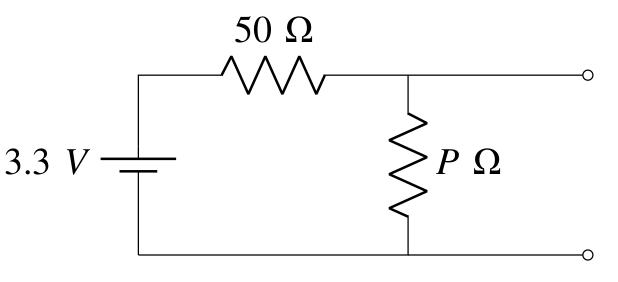
\includegraphics[width=0.6\columnwidth]{figs/Circuit Diagram.png}
    \caption{Circuit Diagram}
    \label{fig:Circuit}
	\end{figure}
\end{frame}
\begin{frame}{Data Acquisition}
	\begin{itemize}
		\item From the above circuit we can see that the voltage across PT-100 sensor is given by,
		\begin{align}
			V_P = 3.3\brak{\frac{P}{P+50}}V
		\end{align} 
		\item As the temperature increases, resistance of the PT-100 sensor increases and hence the voltage across PT-100 sensor $V_P$ increases.
		\item We use an arduino board to read the voltage $V_P$ and a thermomenter to measure the corresponding temperature.
	\end{itemize}
\end{frame}
\section{Regression}
\begin{frame}{Regression Model}
	We model the relation between Voltage $V_P$ and the temperature $T$ as,
	\begin{align}
		V_P(T) = C+BT+AT^2
	\end{align}
Say we collect N data points $(V_{P_1},T_1),(V_{P_2},T_2),\hdots (V_{P_N},T_N)$. Then we can write these N equations as,
	\begin{align}
		\vec{v} &= \vec{X} \vec{n}\\ 
		\myvec{V_{P_1}\\V_{P_2}\\\vdots \\ V_{P_N}} &= \myvec{1& T_1 & T_1^{2}\\ 1& T_2 & T_2^{2}\\ \vdots & \vdots & \vdots  \\ 1& T_N & T_N^{2}} \myvec{C\\ B\\ A}
	\end{align}
\end{frame}
\begin{frame}{Training Data}
    The following table shows the data that is used to train the regression model
	\begin{table}[!ht]
    	\centering
    	%%%%%%%%%%%%%%%%%%%%%%%%%%%%%%%%%%%%%%%%%%%%%%%%%%%%%%%%%%%%%%%%%%%%%%
%%                                                                  %%
%%  This is a LaTeX2e table fragment exported from Gnumeric.        %%
%%                                                                  %%
%%%%%%%%%%%%%%%%%%%%%%%%%%%%%%%%%%%%%%%%%%%%%%%%%%%%%%%%%%%%%%%%%%%%%%

\begin{center}
\begin{tabular}{|c|c|}
\hline
	\textbf{Temperature(in Celcius)}& \textbf{Voltage(in Volts)}\\ \hline
	24	&2.40	\\ \hline
	38	&2.44	\\ \hline
	45	&2.45   \\ \hline
	52	&2.48   \\ \hline
	63	&2.49   \\ \hline
	93	&2.55	\\ \hline
	100	&2.57	\\ \hline
\end{tabular}
\end{center}

    	\caption{Training data}
    	\label{tab:train}
	\end{table}
\end{frame}
\begin{frame}{Regression Model}
	In regression we find the $\vec{n}$ that minimizes the euclidean norm of the error between actual voltage and predicted voltage.
	\begin{align}
		\vec{n_{LS}} = \argmin_{\vec{n}} \norm{\vec{v}-\vec{X}\vec{n}}^2
	\end{align}
	The Least Squares estimate of $\vec{n}$ is given by
	\begin{align}
		\vec{n_{LS}} = (X^{\top}X)^{-1}X^{\top}\vec{v}
	\end{align}
	For the above training data, the least squares estimate that we get is,
	\begin{align}
		\vec{n} = \myvec{2.33483\\ 2.93939\times10^{-3}\\-6.24626\time10^{-6}}
	\end{align}
\end{frame}


\begin{frame}{Plot of Predicted voltage and Training Data}
	\begin{figure}[!ht]
    \centering
    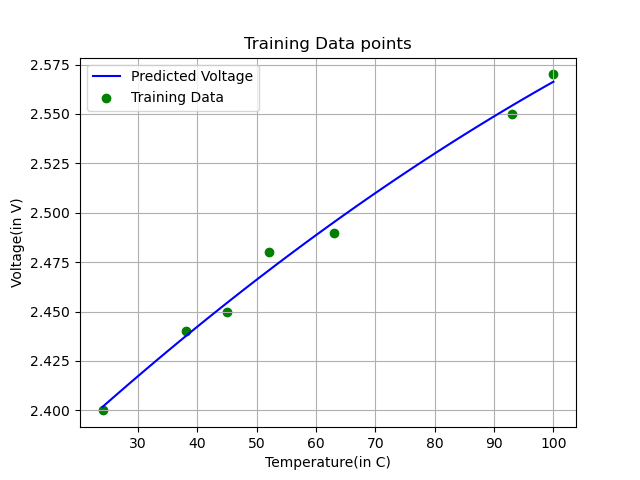
\includegraphics[width=0.6\columnwidth]{figs/Training_Data.png}
    \caption{Training Data}
    \label{fig:T_Data}
	\end{figure}
\end{frame}

\begin{frame}{Validation Data}
    \begin{table}[!ht]
    	\centering
    	%%%%%%%%%%%%%%%%%%%%%%%%%%%%%%%%%%%%%%%%%%%%%%%%%%%%%%%%%%%%%%%%%%%%%%
%%                                                                  %%
%%  This is a LaTeX2e table fragment exported from Gnumeric.        %%
%%                                                                  %%
%%%%%%%%%%%%%%%%%%%%%%%%%%%%%%%%%%%%%%%%%%%%%%%%%%%%%%%%%%%%%%%%%%%%%%

\begin{center}
\begin{tabular}{|c|c|}
\hline
	\textbf{Temperature(in Celcius)}& \textbf{Voltage(in Volts)}\\ \hline
	29	&2.41	\\ \hline
	32	&2.43	\\ \hline
	74	&2.52   \\ \hline
	85	&2.54   \\ \hline
\end{tabular}
\end{center}

    	\caption{Validation data}
    	\label{tab:valid}
	\end{table}
\end{frame}

\begin{frame}{Plot of Predicted voltage and Validation Data}
	\begin{figure}[!ht]
    \centering
    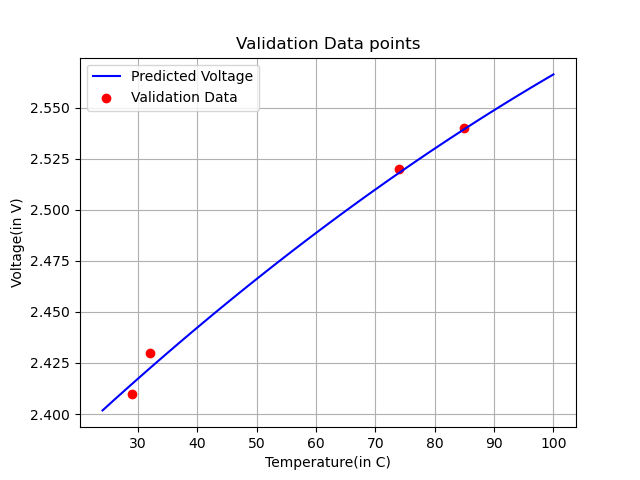
\includegraphics[width=0.6\columnwidth]{figs/Validation_Data.png}
    \caption{Validation Data}
    \label{fig:V_Data}
	\end{figure}
\end{frame}

\section{Conclusion}
\begin{frame}{Conclusion}
	From above plots we can see that Regression is effective in mapping the relation between the voltage across the PT-100 sensor and it's temperature.
\end{frame}

\end{document}
